%File: non-functional-user.tex
%Date: Sat Oct 19 17:06:09 2013 +0800
%Author: Yuxin Wu <ppwwyyxxc@gmail.com>

\subsection{User Management}

\subsubsection{Register Page}

The register page contains an input form, users can only successfully
register an account if:

\begin{itemize}
\itemsep1pt\parskip0pt\parsep0pt
\item
  The username is unique in our database, and contains only letters and
  digits.
\item
  The password is no less than 6 characters, and does not contains
  digits only.
\item
  User repeat the password again correctly.
\item
  User provided a valid email address.
\end{itemize}

After a valid register form is submitted, the server side would again
check the input values. If the form passes, a validation email would
automaticlly be sent to the user with a confirm code. Otherwise, the
client will redirect the user to the original register page again, and
alert about this error message. This process is illustrated well in \figref{register}.

\begin{figure}[H]
  \centering
  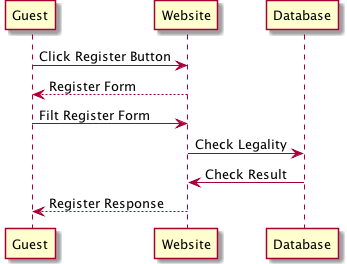
\includegraphics[width=0.6\textwidth]{img/register.png}
  \caption{Registration process\label{fig:register}}
\end{figure}


\subsubsection{Confirm Page}

A link to the confirm page should be attached in the email sent to the
user. An user account will be activated only if:

\begin{itemize}
\itemsep1pt\parskip0pt\parsep0pt
\item
  The email address was registered before but has not been activated
  yet.
\item
  User visits the confirm page within the time constraints.
\item
  A correct confirm code (dependent on this account only) is provided by
  the user.
\end{itemize}

Once an account is activated, user can then edit profile, change
password, and use all the other services provided by Uknow.

\subsubsection{Login/Logout Page}

A visitor will be redirected to login page everytime he/she tries to
visit a restricted resource. In the login page, the user is asked to
provide username together with password. A session is stored in cookie
after a successful login, otherwise, a ``password error'' message will
be displayed. On logging out, this session shall be destroyed and user will be
redirected to the  home page.
The login/logout process is illustrated in \figref{login} and \figref{logout}.
\begin{figure}
\begin{minipage}[b]{0.57\linewidth}
  \centering
  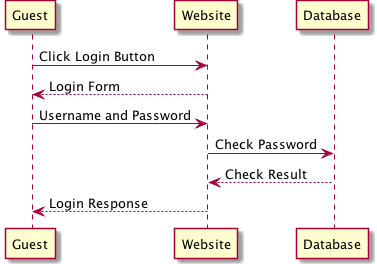
\includegraphics[width=\textwidth]{img/login.png}
  \caption{Login Process \label{fig:login}}
\end{minipage}
\begin{minipage}[b]{0.37\linewidth}
  \centering
  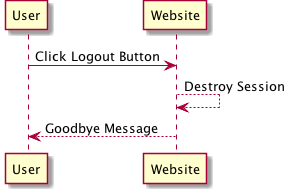
\includegraphics[width=\textwidth]{img/logout.png}
  \caption{Logout Process \label{fig:logout}}
\end{minipage}
\end{figure}



\subsubsection{Profile Page}

User can view and edit the following items:

\begin{itemize}
\itemsep1pt\parskip0pt\parsep0pt
\item
  Avatar, this could be uploaded by user or selected from Gravatar.com
\item
  Nickname, which is displayed in the front page of the site.
\item
  Sex, you know what I mean.
\item
  Age, those under 16 is supposed to be warned before accessing items
  with specific labels.
\item
  Email address, another validation email will be sent if this item is
  changed
\end{itemize}

On the other hand, users should be able to provide access to some social
networking sites for us to collect information including but not limited
to:

\begin{itemize}
\itemsep1pt\parskip0pt\parsep0pt
\item
  Weibo, a twitter-like site in mainland China.
\item
  Renren, a facebook-like site which is very popular among Chinese
  students
\item
  QQ, a MSN-like IM tool running by Tencent
\item
  Tsinghua Netclass, specially provided for Tsinghua student
\end{itemize}

Finally, if user wishes to delete his/her account, a confirm email will
also be sent.

\subsubsection{Change Password}

The password of an account could be changed only if:

\begin{itemize}
\itemsep1pt\parskip0pt\parsep0pt
\item
  The correct old password is provided
\item
  A new valid password.
\item
  The new valid password is typed twice and matched well.
\item
  The link to a confirm page which was emailed to the user was clicked
  within 24h.
\end{itemize}
